\subsection{\NomeBloco}

Um segundo tipo de inversor foi constru\'ido para ser utilizado no bloco Buffer (apresentado na \autoref{secaoBuffer}). Este Inversor apresenta a mesma Tabela Verdade, sinais e circuito do Inversor na \autoref{inversor1}, por\'em com representa{\c c}\~ao em bloco e par\^ametros dos transistores diferentes. A \autoref{fig_inversor2} apresenta a sua representa{\c c}\~ao em bloco, enquanto a \autoref{tab_inversor2} apresenta os par\^ametros de seus componentes.

\begin{figure}[htb]
 \label{fig_inversor2}
 \centering
    \centering
    \caption{Representa{\c c}\~ao em bloco do segundo Inversor } \label{\NomePFig}
    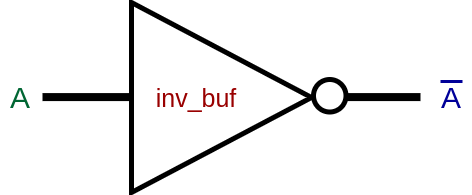
\includegraphics[scale=0.5]{Circuitos/inv_buf_simbolo.png}
    \legend{Fonte: Produzido pelo autor}\end{figure}

Os transistores utilizados no bloco do segundo Inversor apresentam os par\^ametros mostrados na \autoref{\NomeTTab}.

\begin{table}[htbp]
\caption{Sinais do bloco \NomeBloco}
\label{\NomeTTab}
\centering
\begin{tabular}{ccccc}
\toprule
Transistor & W ($\mu$m)  & L ($\mu$m)           & M (n° dispositivos) & S (n° dispositivos)\\
\midrule \midrule
Q1 & 1,2 & 0,18 & 1 & 1\\
\midrule
Q2 & 0,6 & 0,18 & 1 & 1\\
\bottomrule
\end{tabular}
\legend{Fonte: Produzido pelo autor}
\end{table}
\clearpage